%-------------------------------------------------------------------------------
\usetikzlibrary{calc}
%coordinate test point. Use as follows: 	\coordinate (cen) 	 	 at (0,0) (cen) [point];
\tikzset{
	every point/.style = {radius={\pgflinewidth}, opacity=1, draw, solid, fill=white},
	pt/.pic = {
		\begin{pgfonlayer}{foreground}
			\path[every point, #1] circle;
		\end{pgfonlayer}
	},
	point/.style={insert path={pic{pt={#1}}}}, point/.default={},
	point name/.style = {insert path={coordinate (#1)}}
}
%-------------------------------------------------------------------------------

% basic delacations
\pgfdeclarelayer{background}%
\pgfdeclarelayer{foreground}%
\pgfsetlayers{background,main,foreground}%

%Coin Symbol--------------------------------------------------------------------
\tikzset{%
	pics/coin/.style n args={6}{%
		code ={
			\def \coinLineWidth {#1}%
			\def \coinCenDist   {#2}%
			\def \circRad       {#3}%
			\def \circColor     {#4}%
			\def \coinColorL    {#5}%
			\def \coinColor     {#6}%
			\def \signRad       {\circRad*0.20}%
			\def \signRadProp   {0.45}
			\def \signRadExt    {\signRad*\signRadProp}
			\def \signRadOut    {\signRad+\signRadExt}
			\def \signAngle     {30}
			\def \sinSignAngle  {sin(\signAngle)}
			\def \cosSignAngle  {cos(\signAngle)}
			\def \signWidth     {{pow((pow(\signRadOut,2)-pow(\sinSignAngle*\signRad,2)),0.5)-(\cosSignAngle)*\signRad)}}
			
			\def \startIX       {{cos(\signAngle)*\signRad}}
			\def \startIY       {{\sinSignAngle*\signRad}}
			
			\def \startOY       {\startIY}
			\def \signAngleOutS {{atan((\sinSignAngle*\signRad)/pow((pow(\signRadOut,2)-pow(\sinSignAngle*\signRad,2)),0.5))}}
			\def \signAngleOutE {{360-atan((\sinSignAngle*\signRad)/pow((pow(\signRadOut,2)-pow(\sinSignAngle*\signRad,2)),0.5))}}
	%
			\coordinate ()          at ( 0.0     , 0.0);%
			\coordinate (cen)       at ( 0.0     , 0.0);%
			\coordinate (cenB)      at ($(cen)    + ( 0.00,-\coinCenDist)$);%
						
			\node[
				circle,
				draw = \coinColorL,
				fill = \circColor,
				line width = \coinLineWidth,
				minimum size = \circRad,
				inner sep = 0pt,
				outer sep = 0pt,
			](NCD) at (cenB) {};
			
			\node[
				circle,
				draw = \coinColorL,
				fill = \circColor,
				line width = \coinLineWidth,
				minimum size = \circRad,
				inner sep = 0pt,
				outer sep = 0pt,
			](NCU) at (cen) {};
			
%			\draw[ - , line width = \coinLineWidth, black] (NCU.195) -- (NCD.195);
			\draw[-, line width = \coinLineWidth, \coinColorL] (NCU.210) -- (NCD.210);
			\draw[-, line width = \coinLineWidth,\coinColorL] (NCU.225) -- (NCD.225);
			\draw[-, line width = \coinLineWidth, \coinColorL] (NCU.240) -- (NCD.240);
			\draw[-, line width = \coinLineWidth, \coinColorL] (NCU.255) -- (NCD.255);
			\draw[-, line width = \coinLineWidth, \coinColorL] (NCU.270) -- (NCD.270);
			\draw[-, line width = \coinLineWidth, \coinColorL] (NCU.285) -- (NCD.285);
			\draw[-, line width = \coinLineWidth, \coinColorL] (NCU.300) -- (NCD.300);
			\draw[-, line width = \coinLineWidth, \coinColorL] (NCU.315) -- (NCD.315);
			\draw[-, line width = \coinLineWidth, \coinColorL] (NCU.330) -- (NCD.330);
%			\draw[ - , line width = \coinLineWidth, black] (NCU.345) -- (NCD.345);
			
			\draw[
				 - ,
				 line width = \coinLineWidth,
				 \coinColorL,
				 fill = \coinColor
			]
				(\startIX,-\startIY) arc (360-\signAngle:\signAngle:\signRad)
				-- +(\signWidth, 0.0)
				arc (\signAngleOutS:\signAngleOutE:\signRadOut)
				-- (\startIX,-\startIY)
				-- cycle
				;
		}%
		
	} ,%
	pics/coin/.default={1.0pt}{0.1}{1cm}{bg}{black!80!white}{black!90!white}%
}%
%
%\only<1->{%
%\only<1-7>{%
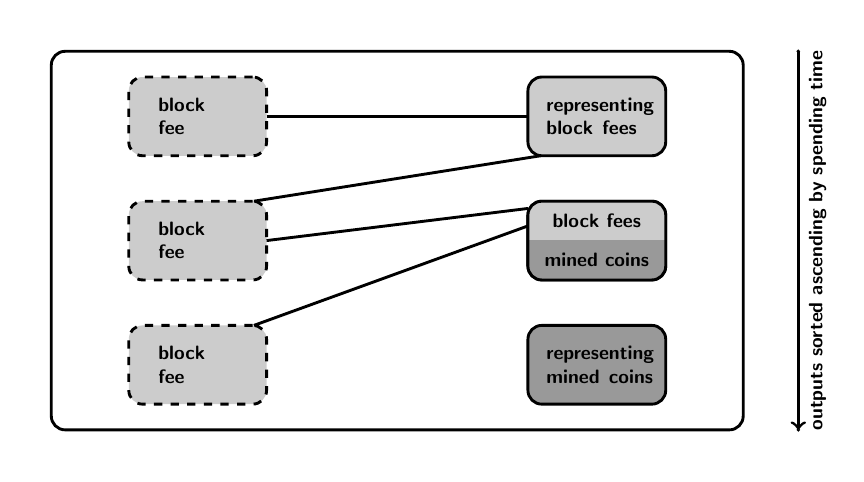
\begin{tikzpicture}[scale=1.0]
	\def \debugPoint   {}%
%	\def \debugPoint   {point}%
	\def \debugPointF  {point}%
	% font settings ############################################################
	\def \fontset      {\scriptsize\sffamily\bfseries}
	% color definition #########################################################
%	\def \colorOut     {jwigreige!50}
%	\def \colorOutH    {jwigreige!25!black}
	\def \colorIn      {black!10!white}
	\def \colorCoin    {white}
	\def \colorCoinY   {jwilightgreen!80!bg}
	\def \colorCoinN   {jwiorange}
	\def \colorCoinUtxoL {black!30!white}
	\def \colorCoinUtxo  {black!40!white}
	% arrow and line definitions ###############################################
	\def \lineW        {1.3pt}
	% width/height definition ##################################################
	\def \picW         {\columnwidth*24/31}%
	\def \picH         {\paperheight*6/31}%
	\def \TDX          {0.3cm}%
	\def \TDY          {0.3cm}%
	
	\def \IPosX        {\picW*3/10}%
	\def \IPosY        {\picH*7/24}%
	
	\def \SPosX        {0.7cm} % sorting position
	
	% tikz styles################################################################
	\tikzstyle{lineIO}       = [
		- ,
		line width = \lineW*0.8,
	]
	\tikzstyle{nodeOuter}    = [
%		draw,
%		rectangle,
%		rounded corners=5pt,
%		solid,
%		line width = \lineW,
%		black,
%		fill=\colorOut,
%		inner sep = 0pt,
%		outer sep = 0pt,
%		text width = \BOW,
%		minimum width = \BOW,
%		minimum height = \BOH*1.075,
		lineIO, 
		solid, 
		%		fill = black!20!white, 
		rounded corners=5pt
	]
	\tikzstyle{nodeInner}    = [
		draw,
		black,
		solid,
		rectangle,
		rounded corners=5pt,
		fill=black!20!white,
		minimum height = 1.0cm,
		minimum width = 1.75cm,
		text width = 1cm,
		lineIO,
		inner sep = 0pt,
		outer sep = 0pt,
	]	
	% coordinates ###############################################################
	% 1 | 2 | 3 | 4 | 5 | 6 | 7 | 8 | 9 | 10 | 11 | 12 | 13 | 14 |
	% A | B | C | D | E | F | G | H | I |  J |  K |  L |  M |  N |
	
	\coordinate (cen)    at ($( 0.0, 0.0) + ( 0.0        , 0.0         )$) (cen)   [\debugPoint];%
	\coordinate (Tcen)   at ($(cen)       + (-\picW*0.25 , 0.0         )$) (cen)   [\debugPoint];%
	
	\coordinate (PLU)    at ($(Tcen)      + (-\picW*0.5  , \picH*0.5   )$) (PLU)   [\debugPoint];%
	\coordinate (PLD)    at ($(Tcen)      + (-\picW*0.5  ,-\picH*0.5   )$) (PLD)   [\debugPoint];%
	\coordinate (PRU)    at ($(Tcen)      + ( \picW*0.5  , \picH*0.5   )$) (PRU)   [\debugPoint];%
	\coordinate (PRD)    at ($(Tcen)      + ( \picW*0.5  ,-\picH*0.5   )$) (PRD)   [\debugPoint];%
	
	\coordinate (TLU)    at ($(PLU)       + ( \TDX*1.0   ,-\TDY*1.0    )$) (TLU)   [\debugPoint];%
	\coordinate (TLD)    at ($(PLD)       + ( \TDX*1.0   , \TDY*1.0    )$) (TLD)   [\debugPoint];%
	\coordinate (TRU)    at ($(PRU)       + (-\TDX*1.0   ,-\TDY*1.0    )$) (TRU)   [\debugPoint];%
	\coordinate (TRD)    at ($(PRD)       + (-\TDX*1.0   , \TDY*1.0    )$) (TRD)   [\debugPoint];%
		
	\coordinate (IA)     at ($(Tcen)      + (-\IPosX*0.9 , \IPosY*1.0  )$) (IA)    [\debugPoint];%
	\coordinate (IB)     at ($(Tcen)      + (-\IPosX*0.9 , \IPosY*0.0  )$) (IB)    [\debugPoint];%
	\coordinate (IC)     at ($(Tcen)      + (-\IPosX*0.9 ,-\IPosY*1.0  )$) (IC)    [\debugPoint];%
	
	\coordinate (OA)     at ($(Tcen)      + ( \IPosX*0.9 , \IPosY*1.0  )$) (OA)    [\debugPoint];%
	\coordinate (OB)     at ($(Tcen)      + ( \IPosX*0.9 , \IPosY*0.0  )$) (OB)    [\debugPoint];%
	\coordinate (OC)     at ($(Tcen)      + ( \IPosX*0.9 ,-\IPosY*1.0  )$) (OC)    [\debugPoint];%
	
	%for sorting arrow
	\coordinate (SU)     at ($(TRU)       + ( \SPosX*1.0 , 0.0         )$) (SU)    [\debugPointF];%
	\coordinate (SD)     at ($(TRD)       + ( \SPosX*1.0 , 0.0         )$) (SD)    [\debugPointF];%
	
	%clipping
%	\clip ($(PLD) + ( 0.0 , 0.0)$) rectangle ($(PRU) + ( 0.0 ,-0.1)$);
	%basic picture
	
	% Slide numbering helper
	
%	\node[,] () at ($(cen) + ( 0.00, 0.00)$) {\fontset{}\large\textbf{1}};
%	\node[,] () at ($(cen) + ( 0.00, 0.00)$) {\fontset{}\large\textbf{2}};	
%	\node[,] () at ($(cen) + ( 0.00, 0.00)$) {\fontset{}\large\textbf{3}};
%	\node[,] () at ($(cen) + ( 0.00, 0.00)$) {\fontset{}\large\textbf{4}};
%	\node[,] () at ($(cen) + ( 0.00, 0.00)$) {\fontset{}\large\textbf{5}};
%	\node[,] () at ($(cen) + ( 0.00, 0.00)$) {\fontset{}\large\textbf{6}};
%	\node[,] () at ($(cen) + ( 0.00, 0.00)$) {\fontset{}\large\textbf{7}};
%	\node[,] () at ($(cen) + ( 0.00, 0.00)$) {\fontset{}\large\textbf{8}};
							
	%Vertical Lines============================================================%
	
	%Nodes=====================================================================%	
%	fill=black!20!white,
	\linespread{0.7}
	\draw[nodeOuter] (TLD) -- (TLU) -- (TRU) -- (TRD) -- cycle;
	%fee nodes as "inputs"
	\node[nodeInner, dashed](NIA) at (IA) {\fontset{}block fee};
	\node[nodeInner, dashed](NIB) at (IB) {\fontset{}block fee};
	\node[nodeInner, dashed](NIC) at (IC) {\fontset{}block fee};
	%outputs nodes, fee only node
	\node[nodeInner](NOA) at (OA) {};
	\node[nodeInner, draw=none, fill=none, align=left](NOAT) at ($(NOA.center) + (-4pt, 0pt)$) {\fontset{}representing\\\fontset{}\mbox{block fees}};
	%outputs nodes, partly fee/coins node
	\node[nodeInner,fill=none](NOB)  at (OB) {};
	\filldraw[black!20!white] (NOB.180) [rounded corners=5pt] -- (NOB.north west) -- (NOB.north east) -- (NOB.0) -- cycle;
	\filldraw[black!20!white] (NOB.180)  -- (NOB.170) -- (NOB.10) -- (NOB.0) -- cycle;
	\filldraw[black!40!white] (NOB.180) [rounded corners=5pt] -- (NOB.south west) -- (NOB.south east) -- (NOB.0) -- cycle;
	%coin only node
	\filldraw[black!40!white] (NOB.180)  -- (NOB.190) -- (NOB.350) -- (NOB.0) -- cycle;
	\node[nodeInner,fill=none](NOBB) at (OB) {};
	
	\node[ draw=none, fill=none](NOBTA) at ($(NOB.center) + (0pt, 0.25cm)$) {\fontset{}\mbox{block fees}};
	\node[ draw=none, fill=none](NOBTB) at ($(NOB.center) + (0pt,-0.25cm)$) {\fontset{}\mbox{mined coins}};
	\node[nodeInner,fill=black!40!white,](NOC) at (OC) {};
	\node[nodeInner, draw=none, fill=none](NOCT) at ($(NOC.center) + (-4pt, 0.00)$) {\fontset{}representing\\\fontset{}\mbox{mined coins}};
	
	%Arrows depending on nodes=================================================%
	\draw[lineIO,] (NIA.00) .. controls ($(NIA.00) + ( 0.00, 0.00)$) and ($(NOA.180) + ( 0.00, 0.00)$) .. (NOA.180);
	\draw[lineIO,] (NIB.35) .. controls ($(NIB.35) + ( 0.00, 0.00)$) and ($(NOA.215) + ( 0.00, 0.00)$) .. (NOA.215);
	\draw[lineIO,] (NIB.00) .. controls ($(NIB.00) + ( 0.00, 0.00)$) and ($(NOB.155) + ( 0.00, 0.00)$) .. (NOB.155);
	\draw[lineIO,] (NIC.35) .. controls ($(NIC.35) + ( 0.00, 0.00)$) and ($(NOB.168) + ( 0.00, 0.00)$) .. (NOB.168);
	
	\draw[lineIO, solid, ->] (SU) -- node [below, rotate=90] {\fontset{}outputs sorted ascending by spending time} (SD);
	
	%Coin Symbols==============================================================%
	%TxA-----------------------------------------------------------------------%
%	\pic[ ,] () at ($(NBAUBL.east) + (-\BOH*0.125,-\BOH*0.0375)$) {coin={0.7pt}{0.05}{\BOH*0.12}{\colorCoin} {black!80!white}{black!90!white}};

	
	%Counter Node==============================================================%
%	\pic[  ] ()        at ($(BCount) + ( \BOH*0.225/2, 0.05)$) {coin={1.0pt}{0.07}{\BOH*0.225}{\colorCoinY}{black!90!white}{black!100!white}};
\end{tikzpicture}
%}%